\documentclass[11pt,oneside]{scrbook}
\usepackage[a4paper,margin=2.4cm,marginparwidth=1.8cm,marginparsep=0.4cm]{geometry}
\usepackage{../common/rlstudy}
\usepackage[ruled,vlined,linesnumbered]{algorithm2e}

\title{{\color{rlblue}\textbf{Week 03} \\ \Huge Monte Carlo Methods}}
\author{STUDY-RL --- a self-paced Deep RL curriculum}
\date{\today}

\begin{document}
\maketitle
\tableofcontents
\newpage

% =============================================================================
\chapter*{Learning objectives}
\addcontentsline{toc}{chapter}{Learning objectives}

% Teaching companion: a small example before the full lecture.
\noindent\textbf{Study companion.} Read \texttt{teaching\_guide.md} in this
folder for step-by-step examples, an analogy with its limits, and self-checks.
Then use \texttt{workbook.ipynb} to implement and vary the calculations.
\par\medskip

\begin{keyidea}
By the end of this week you will be able to:
\begin{enumerate}\setlength\itemsep{2pt}
  \item Distinguish \emph{first-visit} and \emph{every-visit} Monte Carlo
        prediction; prove that both are unbiased estimators of $V^\Policy$
        and that first-visit has lower variance in dependent samples.
  \item Implement \emph{on-policy MC control with an $\epsilon$-soft policy}
        and reproduce Sutton \& Barto's figure 5.2 on Blackjack.
  \item Derive the \emph{ordinary} and \emph{weighted} importance-sampling
        estimators for off-policy MC and compute their variance.
  \item Identify when an off-policy estimator is consistent and what
        \emph{coverage} assumption is required for the importance weights to
        be defined.
  \item Apply off-policy MC to a delayed-feedback \emph{recruitment funnel} as
        a toy applied matching task.
\end{enumerate}
\end{keyidea}

% =============================================================================
\chapter{Motivation \& intuition}

The big idea this week is replacing the \emph{expectation} in the Bellman
equation by a \emph{sample mean}. Last week we had the model and could
exhaustively compute $\sum_{s',r} p(s',r\mid s,a)[r + \Disc V(s')]$. Now
suppose the only thing we have is the ability to \emph{generate} trajectories:
sequence of $(S_t, A_t, R_{t+1})$ tuples by interacting with the environment.
The law of large numbers tells us that an average of returns
$\Ret^{(1)},\dots,\Ret^{(N)}$ obtained from $N$ independent episodes converges
to $V^\Policy(s_0)$. That is Monte Carlo policy evaluation in one sentence.

\begin{intuition}
Monte Carlo methods trade \emph{model knowledge} for \emph{samples}. They are
the dynamical-systems equivalent of estimating $\pi$ by throwing darts: noisy,
embarrassingly parallel, and convergent at rate $1/\sqrt{N}$ rather than
$\Disc^k$. The variance penalty is real; the modelling freedom is enormous.
\end{intuition}

\paragraph{Why MC and not TD?} TD methods (Week 4) combine the Bellman
recursion with sampling and so reduce variance \emph{at the cost of bias} (the
TD target uses an old, biased value estimate). MC keeps the full episodic
return; it is unbiased but high variance. For tasks with short episodes and
sparse terminal rewards (e.g.\ Blackjack, or the recruitment funnel later in
this lecture) MC is often the cleaner choice.

\begin{pitfall}
\textbf{MC and continuing tasks.} If $\Disc=1$ and episodes do not terminate
almost surely, the return is undefined and the MC estimator is degenerate.
Either impose a truncation (with bias) or use a $\Disc<1$ formulation (also
biased, but in a way you can control). Average-reward MC exists and is
discussed in Mahadevan (1996) and Bertsekas--Tsitsiklis (1996, Ch.\ 7).
\end{pitfall}

% =============================================================================
\chapter{Mathematical formulation}

\section{MC policy evaluation}

\begin{definition}[First-visit MC estimator]
Given $N$ independent episodes generated by $\Policy$, let $\Ret^{(i)}_s$ be
the return following the \emph{first} visit to state $s$ in episode $i$ (skip
episodes that never visit $s$). Then
\[
\hat V_{\mathrm{FV}}(s) = \frac{1}{N_s} \sum_{i:\,s\in\tau_i} \Ret^{(i)}_s,
\]
where $N_s$ is the number of episodes in which $s$ was visited at least once.
\end{definition}

\begin{definition}[Every-visit MC estimator]
$\hat V_{\mathrm{EV}}(s) = \tfrac{1}{M_s}\sum_{(\text{visits to } s)} \Ret_{\text{at that visit}}$,
where $M_s$ is the total number of visits, summed over episodes.
\end{definition}

\begin{theorem}
$\hat V_{\mathrm{FV}}$, conditional on at least one contributing episode,
is an unbiased estimator of $V^\Policy(s)$ for independent episodes under
a fixed stationary Markov policy and integrable returns;
$\hat V_{\mathrm{EV}}$ is biased in finite samples but consistent.
\end{theorem}

\begin{proof}[Sketch]
For first-visit: the random variable $\Ret_s^{(i)}$ has expectation $V^\Policy(s)$
by definition of $V^\Policy$, and the $\Ret^{(i)}_s$ across episodes are i.i.d.,
so the sample mean is unbiased. For every-visit, repeated visits within the
same episode can share environment randomness. Correlation alone does not
prove bias; the random visit-count denominator is also coupled to the returns.
Under suitable episodic moment assumptions, a law of large numbers across
independent episodes gives consistency of the ratio of total returns to
total visits. Within-episode dependence need not vanish. See Singh \& Sutton 1996. \qedhere
\end{proof}

\section{On-policy MC control with $\epsilon$-soft policies}

We follow Sutton \& Barto's GPI template: alternate
(i) MC policy evaluation of $\Qfn^\Policy$ and
(ii) policy improvement to an $\epsilon$-greedy update of $\Policy$:
\[
\Policy_{\text{new}}(a\mid s) = \begin{cases}
1 - \epsilon + \tfrac{\epsilon}{|\Actions|} & \text{if } a = \argmax_a \Qfn(s,a),\\
\tfrac{\epsilon}{|\Actions|} & \text{otherwise.}
\end{cases}
\]
A positive $\epsilon$ gives each action positive probability at visited
states. Coverage of state-action pairs additionally requires reachability
from the start distribution and sufficiently many visits; unreachable
states are not made reachable by action randomisation.

\begin{theorem}[Policy improvement for $\epsilon$-soft policies]
Let $\Policy$ be $\epsilon$-soft and let $\Policy'$ be the $\epsilon$-soft
greedification of $\Qfn^\Policy$ above. Then $V^{\Policy'}(s) \ge V^\Policy(s)$
for all $s$.
\end{theorem}

\begin{proof}[Idea]
Same telescoping argument as Week 2 with the modification that the maximum is
taken \emph{within} the class of $\epsilon$-soft policies; the
$\epsilon/|\Actions|$ slack in each action just adds a constant offset that
cancels in the telescope. \qedhere
\end{proof}

\section{Off-policy MC: importance sampling}

Now the data are generated by a \emph{behaviour} policy $b$, but we want to
estimate the value of a different \emph{target} policy $\Policy$. The
\emph{coverage} assumption $b(a\mid s)>0$ whenever $\Policy(a\mid s)>0$ is
required; otherwise the importance weights are undefined.

\begin{definition}[Importance-weight for a trajectory $\tau$]
\[
\rho_\tau \defeq \prod_{t=0}^{T-1} \frac{\Policy(A_t\mid S_t)}{b(A_t\mid S_t)}.
\]
\end{definition}

\begin{theorem}[Ordinary IS]
\[
\hat V_{\mathrm{OIS}}(\Policy)
   = \frac{1}{N}\sum_{i=1}^N \rho_{\tau_i} \Ret^{(i)}
\]
is an \emph{unbiased} estimator of $V^\Policy(s_0)$ under coverage, but its
variance can be infinite.
\end{theorem}

\begin{proof}[Sketch]
$\E_b[\rho_\tau f(\tau)] = \sum_\tau b(\tau) \frac{\Policy(\tau)}{b(\tau)} f(\tau)
= \E_\Policy[f(\tau)]$ for any bounded $f$, by direct change of measure.
Set $f(\tau)=G(\tau)$. Variance:
$\Var_b[\rho_\tau G] = \E_\Policy[\rho_\tau G^2] - V^\Policy(s_0)^2$ where
$\rho_\tau$ inside the $\Policy$-expectation is now upper-bounded by
$(\max_{s,a} \Policy/b)^T$; for $T$ large this can blow up exponentially. \qedhere
\end{proof}

\begin{theorem}[Weighted IS]
\[
\hat V_{\mathrm{WIS}}(\Policy) = \frac{\sum_i \rho_{\tau_i} \Ret^{(i)}}{\sum_i \rho_{\tau_i}}
\]
is \emph{biased} ($\E[\hat V_{\mathrm{WIS}}] \ne V^\Policy$ in finite samples)
but consistent under coverage and the required integrability assumptions.
It is defined only when $\sum_i\rho_{\tau_i}>0$. With nonnegative weights
and returns bounded in $[L,U]$, the estimate also lies in $[L,U]$.
\end{theorem}

\begin{remark}[Practical guidance]
WIS often reduces sensitivity to a fluctuating total weight, but neither
variance nor mean-squared-error dominance over OIS is universal. Compare
estimator uncertainty and effective sample size, and check coverage.
The companion teaching guide gives an exact two-action counterexample.
\end{remark}

\paragraph{Per-decision IS.}
Trajectory-level $\rho_\tau$ is exponentially bad in $T$. \emph{Per-decision}
IS noticing that the reward at time $t$ depends only on $A_0,\dots,A_t$:
\[
\hat V_{\mathrm{PD}}(\Policy) = \frac{1}{N}\sum_i \sum_{t=0}^{T-1}
   \Disc^t \, \rho^{(i)}_{0:t} \, R^{(i)}_{t+1},
\quad
\rho_{0:t} = \prod_{k=0}^{t}\frac{\Policy(A_k\mid S_k)}{b(A_k\mid S_k)}.
\]
Per-decision IS has the same expectation and (usually) much lower variance.
See Precup, Sutton, Singh (2000) for the full proof.

% =============================================================================
\chapter{Algorithms}

\begin{algorithm}[H]
\SetAlgoLined
\KwIn{$\Policy$, $\Disc$, $N$ episodes.}
Initialise $\hat V(s) \gets 0$, $N_s\gets 0$ for all $s$.\;
\For{$i = 1,\dots,N$}{
  Generate an episode $S_0, A_0, R_1, \dots, S_T$ following $\Policy$.\;
  $G\gets 0$\;
  \For{$t = T-1, T-2, \dots, 0$}{
    $G \gets R_{t+1} + \Disc G$\;
    \If{$S_t \notin \{S_0,\dots,S_{t-1}\}$ (first-visit)}{
      $N_{S_t} \mathrel{+}= 1$;
      $\hat V(S_t) \mathrel{+}= (G - \hat V(S_t)) / N_{S_t}$\;
    }
  }
}
\caption{First-visit MC policy evaluation.}
\end{algorithm}

\begin{algorithm}[H]
\SetAlgoLined
\KwIn{$\Disc$, $\epsilon$, $N$ episodes.}
Initialise $\Qfn(s,a)\gets 0$, $N_{s,a}\gets 0$; arbitrary $\Policy$.\;
\For{$i=1,\dots,N$}{
  Generate an episode following the $\epsilon$-soft $\Policy$.\;
  $G\gets 0$\;
  \For{$t = T-1, \dots, 0$}{
    $G \gets R_{t+1} + \Disc G$;
    $N_{S_t,A_t}\mathrel{+}= 1$;
    $\Qfn(S_t,A_t) \mathrel{+}= (G - \Qfn(S_t,A_t))/N_{S_t,A_t}$\;
  }
  Update $\Policy$ to be $\epsilon$-soft greedification of $\Qfn$\;
}
\caption{On-policy every-visit MC control with $\epsilon$-soft policies.}
\end{algorithm}

\begin{algorithm}[H]
\SetAlgoLined
\KwIn{behaviour $b$, target $\Policy$, $\Disc$, $N$ episodes.}
\For{$i=1,\dots,N$}{
  Generate episode $\tau_i$ under $b$; compute $\Ret^{(i)}$ and
  $\rho_{\tau_i} = \prod_t \Policy(A_t\mid S_t)/b(A_t\mid S_t)$.\;
}
\Return $\hat V_{\mathrm{OIS}} = \tfrac{1}{N}\sum_i \rho_{\tau_i}\Ret^{(i)}$\;
\Return $\hat V_{\mathrm{WIS}} = \sum_i \rho_{\tau_i}\Ret^{(i)} / \sum_i \rho_{\tau_i}$\;
\caption{Off-policy MC via importance sampling.}
\end{algorithm}

\begin{pitfall}
\textbf{Forgetting coverage.} If $b(a\mid s)=0$ on a state-action pair where
$\Policy(a\mid s)>0$, the importance weight is $\frac{\Policy}{0}$ --- the
estimator silently returns NaN or $\infty$. Check the support of the full target and logging policies before doing IS;
positive propensities in observed rows alone cannot reveal unsupported
actions that never appear in the data. The bug is easiest to introduce when the behaviour
policy is a deterministic logged policy.
\end{pitfall}

% =============================================================================
\chapter{Implementation walkthrough}

The Blackjack environment is faithful to Sutton \& Barto Example 5.1.

\begin{codebox}
\begin{minted}{python}
# project/blackjack.py (excerpt)
@dataclass
class BlackjackEnv:
    seed: int = 0
    def reset(self, seed=None):
        if seed is not None: self.rng = np.random.default_rng(seed)
        self.player = [_draw_card(self.rng), _draw_card(self.rng)]
        self.dealer = [_draw_card(self.rng), _draw_card(self.rng)]
        while _hand_value(self.player)[0] < 12:
            self.player.append(_draw_card(self.rng))
        self.done = False
        return self._obs()
\end{minted}
\end{codebox}

The off-policy estimator implementation deliberately keeps the
trajectory-level $\rho$ explicit so you can inspect it in the workbook:

\begin{codebox}
\begin{minted}{python}
# project/solutions.py (excerpt)
def exercise_5_weighted_is(rewards, target_prob, logged_prob):
    r  = np.asarray(rewards, dtype=float)
    w  = np.asarray(target_prob) / np.maximum(np.asarray(logged_prob), 1e-12)
    return float((w * r).sum() / max(w.sum(), 1e-12))
\end{minted}
\end{codebox}

% =============================================================================
\chapter{Empirical results}

\begin{figure}[ht]\centering
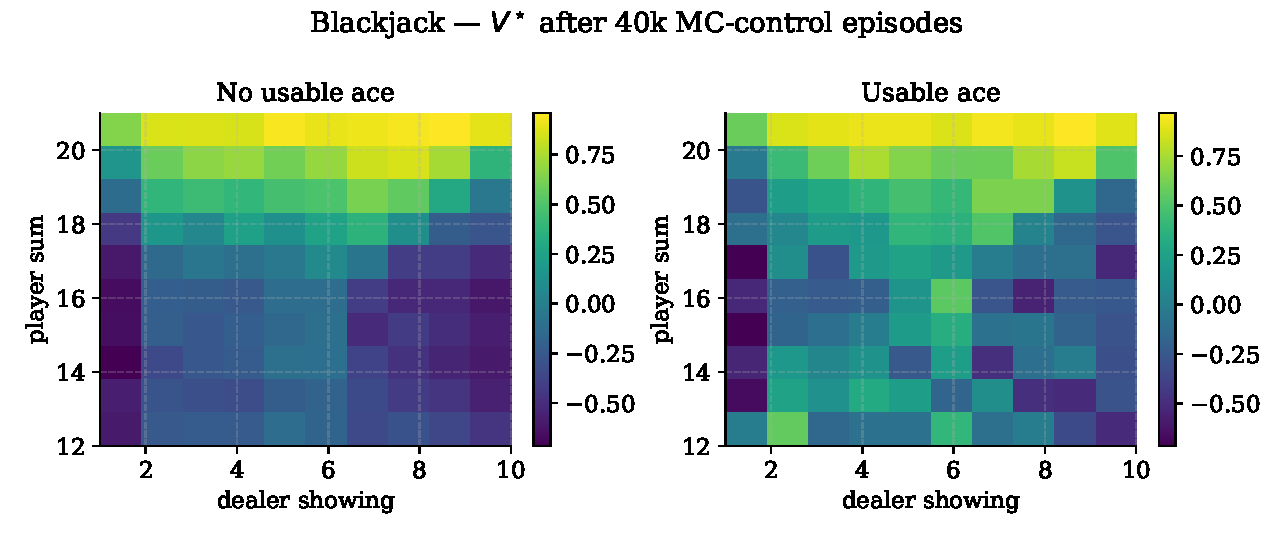
\includegraphics[width=0.92\linewidth]{figs/fig_blackjack_value.pdf}
\caption{Estimated optimal value function on Blackjack after 40k MC-control
episodes (with $\epsilon=0.1$). The left panel is for hands without a usable
ace, the right panel for hands with one. The shapes match Sutton \& Barto's
figure 5.2 (1998).}
\end{figure}

\begin{figure}[ht]\centering
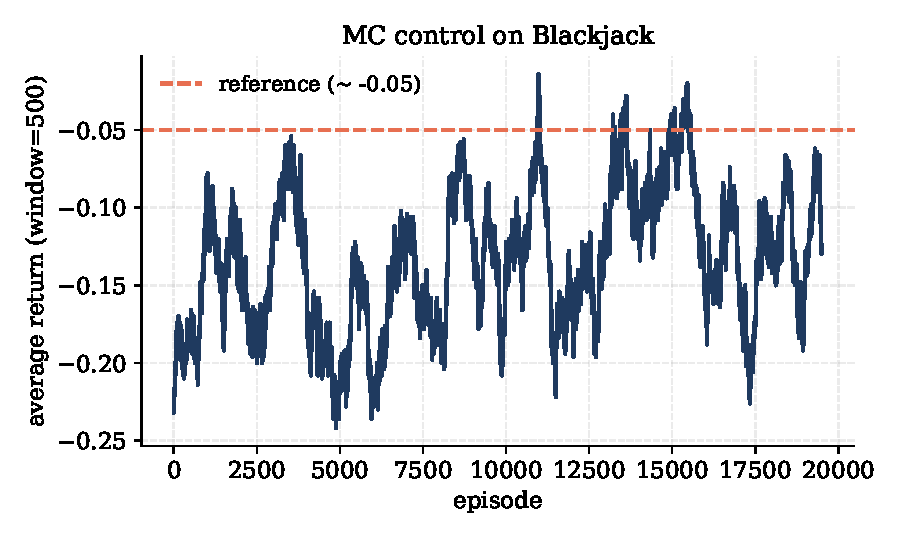
\includegraphics[width=0.92\linewidth]{figs/fig_blackjack_curve.pdf}
\caption{500-episode rolling average of MC-control return on Blackjack.}
\end{figure}

\begin{figure}[ht]\centering
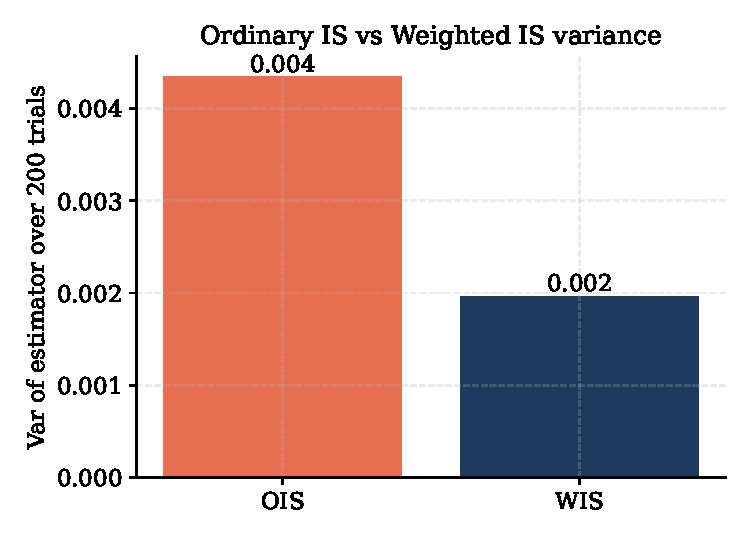
\includegraphics[width=0.55\linewidth]{figs/fig_is_vs_wis.pdf}
\caption{Variance of OIS vs WIS over 200 independent trials of a tiny
two-arm Bernoulli bandit with $\pi=[0.9,0.1]$, $b=[0.5,0.5]$. WIS is many
times lower-variance even with weights bounded by 1.8.}
\end{figure}

% =============================================================================
\chapter{Safety angle}

\begin{safetyangle}
\textbf{Off-policy evaluation is the only safe way to roll out a new policy
in matching.} Three failure modes:

\begin{enumerate}\setlength\itemsep{2pt}
  \item \emph{Coverage holes.} If the production behaviour policy never
        routed certain lead-types to certain brokers, the OIS / WIS / DR
        estimates of any policy that \emph{does} route there have infinite
        variance and you cannot bound the deployment risk.
        Mitigation: \emph{forced exploration budget} (a small $\epsilon$ of
        uniform routing) baked into the production policy so logs cover the
        action space.
  \item \emph{Tail importance weights.} A single huge $\rho_\tau$ dominates
        the OIS estimate. Clip the weights, or use WIS, or use the SWITCH
        / SNIPS estimators (Swaminathan \& Joachims 2015). The bias you take
        on is much smaller than the variance you remove.
  \item \emph{Reward shaping under delay.} Recruitment outcomes arrive weeks
        later; if your training pipeline drops not-yet-realised rewards as
        zero, you bias the evaluator. Use censored-likelihood models
        (Chapelle 2014; \texttt{deeprl\_core\_sota.md} \S 12).
\end{enumerate}

\paragraph{Citations.}
Thomas \& Brunskill, \textsc{Data-Efficient Off-Policy Policy Evaluation for
Reinforcement Learning} (ICML 2016) --- the canonical reference for
\emph{high-confidence} off-policy policy evaluation, which gives you
$1-\delta$ lower bounds on the value of a target policy and is the right
tool when deploying RL to a high-stakes domain.
\end{safetyangle}

% =============================================================================
\chapter{Matching application}

\begin{matching}
\textbf{Recruitment delayed-feedback funnel.}
A candidate moves through 4 stages: screening, interview, offer, outcome.
Action at each stage is ADVANCE or REJECT. Reward is +1 if the hire
materialises (only at the terminal stage); 0 otherwise.

\paragraph{Why MC?} Episodes are short (4 transitions max), terminal, and the
reward signal is fundamentally trajectory-level. There is no value in
bootstrapping a TD target from a halfway-formed $\hat V$; just take the full
return.

\paragraph{Off-policy evaluation in production.} The current ATS routing
policy logs $(x_t, a_t, r_T)$ triples. To compare a candidate policy $\Policy$
without an A/B test, we use WIS over the logs. Two requirements:
\begin{enumerate}\setlength\itemsep{1pt}
  \item Log propensities $b(a\mid x)$ at the time of action, not at
        analysis time. (Logging the action alone is not enough --- if the
        production rules change between data collection and analysis you
        cannot reconstruct $b$.)
  \item Inject a forced-exploration budget into the production policy so
        $b > 0$ on every reasonable $(x, a)$. Coverage is the price of
        admission to off-policy evaluation.
\end{enumerate}

\paragraph{synthetic insurance parallel.} The same scaffold works for synthetic insurance's
lead-broker matcher with the funnel reinterpreted as: contact attempt $\to$
quote produced $\to$ policy bound $\to$ renewed. Long horizons + delayed
rewards give per-decision IS its single most useful application.
\end{matching}

% =============================================================================
\chapter{Exercises}

See \texttt{workbook.ipynb}:
\begin{enumerate}[label={},leftmargin=0pt,labelsep=0pt]\setlength\itemsep{2pt}
  \item \textbf{Ex.\ 1 ($\star$).} First-visit returns from a sample
        trajectory.
  \item \textbf{Ex.\ 2 ($\star$).} Every-visit MC prediction for a fixed
        Blackjack policy (``always stick'').
  \item \textbf{Ex.\ 3 ($\star\star$).} On-policy MC control with
        $\epsilon$-soft policies; reproduce figure 5.2.
  \item \textbf{Ex.\ 4 ($\star\star$).} Ordinary importance sampling.
  \item \textbf{Ex.\ 5 ($\star\star$).} Weighted importance sampling.
  \item \textbf{Ex.\ 6 ($\star\star$).} Empirical variance comparison
        OIS vs WIS.
  \item \textbf{Ex.\ 7 ($\star\star\star$, applied --- matching).}
        Off-policy MC on the recruitment funnel.
  \item \textbf{Ex.\ 8 ($\star\star$).} Verify the bound
        $\Var(w\cdot r) \le w_{\max}^2 \E[r^2]$.
\end{enumerate}

% =============================================================================
\chapter{Further reading}

\texttt{extended\_reading.pdf} unpacks Robbins--Monro (1951), Singh \& Sutton
(1996), Precup-Sutton-Singh (2000), Thomas-Brunskill (2016), and Joachims-
Swaminathan-de Rijke (2018, BanditNet). Source material in
\verb|research/bandits_matching_sota.md| \S 3 and Sutton \& Barto Chapter 5.

\end{document}
